\documentclass[10pt]{beamer}

\usetheme[progressbar=frametitle]{metropolis}
\usepackage{appendixnumberbeamer}
\usepackage{emoji}
\usepackage{booktabs}
\usepackage[scale=2]{ccicons}

\usepackage{pgfplots}
\usepgfplotslibrary{dateplot}

\usepackage{xspace}
\newcommand{\themename}{\textbf{\textsc{metropolis}}\xspace}

\title{Output Dynamics in Real-Business-Cycle Models}
\subtitle{Timothy Cogley and James M. Nason}
\date{\today}

\author{Zixuan, Huixin, Rémi}
\institute{M2 ETE Macroeconomics 2}
% \titlegraphic{%
%     
\includegraphics[width=.3\textwidth]{figures/TSE_Logo_2019.png}\hfill
% }

% \makeatletter
% \setbeamertemplate{title page}{
%   \begin{minipage}[b][\paperheight]{\textwidth}
%     \vfill%
%     \ifx\inserttitle\@empty\else\usebeamertemplate*{title}\fi
%     \ifx\insertsubtitle\@empty\else\usebeamertemplate*{subtitle}\fi
%     \usebeamertemplate*{title separator}
%     \ifx\beamer@shortauthor\@empty\else\usebeamertemplate*{author}\fi
%     \ifx\insertdate\@empty\else\usebeamertemplate*{date}\fi
%     \ifx\insertinstitute\@empty\else\usebeamertemplate*{institute}\fi
%     \vfill
%     \ifx\inserttitlegraphic\@empty\else\inserttitlegraphic\fi
%     \vspace*{1cm}
%   \end{minipage}
% }
% \makeatother

\begin{document}

\maketitle

\begin{frame}{Table of contents}
    \setbeamertemplate{section in toc}[sections numbered]
    \tableofcontents%[hideallsubsections]
\end{frame}

\section{Introduction}

\begin{frame}{Introduction}
    \textit{Are RBC models consistent with output dynamics stylized facts?}\\
    $\Rightarrow$ Compare \alert{output dynamics} in the theoretical RBC model literature and \alert{stylized facts} in the output dynamics analysis\\[1em]

    \begin{itemize}
        \item Stylized fact \#1: \alert{Autocorrelation} for output growth
              \begin{itemize}
                  \item Short horizons: \textbf{Positive and significant}
                  \item Long horizons: \textbf{Negative but insignificant}
              \end{itemize}
    \end{itemize}
    \begin{figure}
        \centering
        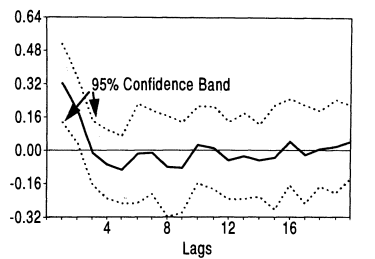
\includegraphics[width=5cm]{figures/sf1.png}
        \caption{Autocorrelation function for output growth}
    \end{figure}
\end{frame}

\begin{frame}
    \begin{itemize}
        \setlength\itemsep{1em}
        \item Stylized fact \#2: \alert{Impulse-response functions} of output
              \begin{itemize}
                  \item \textbf{Permanent shock} $\varepsilon_z$: Output $\uparrow$ then reaches a plateau
                  \item \textbf{Transitory shock} $\varepsilon_g$: Output $\uparrow$ then goes back to stochastic trend
                  \item Variation in GNP growth: mainly due to transitory fluctuation
                  \item[$\Rightarrow$] GNP: important \alert{trend-reverting component}
              \end{itemize}
    \end{itemize}
    \begin{figure}
        \centering
        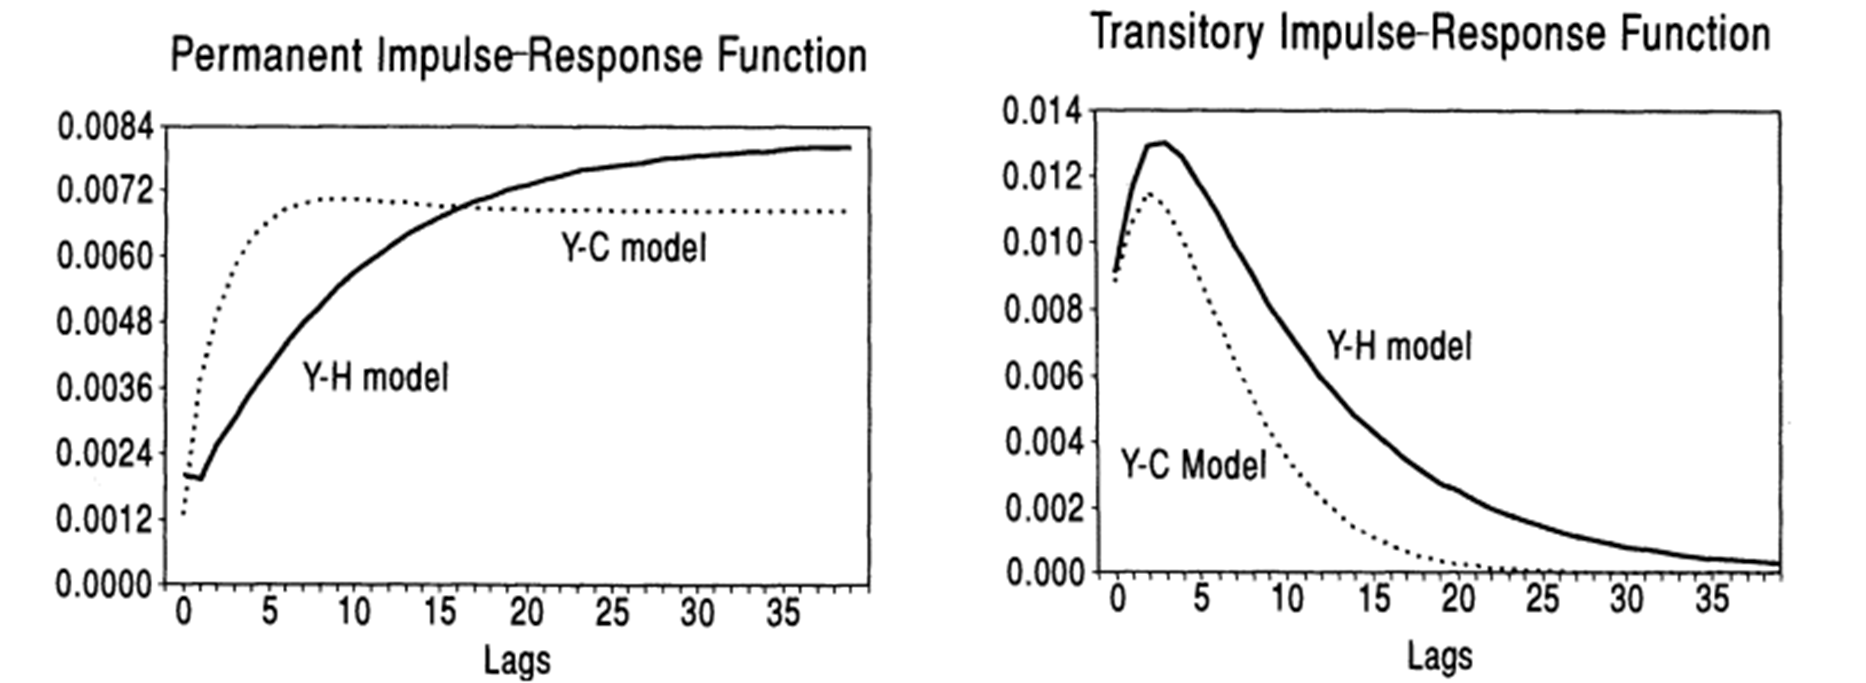
\includegraphics[width=10cm]{figures/sf2.png}
        \caption{Impulse-response functions for output growth}
    \end{figure}
\end{frame}

\begin{frame}
    \begin{itemize}
        \setlength\itemsep{1em}
        \item \alert{Theoretical} part: 3 models
              \begin{enumerate}
                  \item Baseline RBC
                  \item Baseline RBC + capital adjustment cost
                  \item Baseline RBC + labor adjusment cost
              \end{enumerate}
        \item Models examination:
              \begin{itemize}
                  \item For each model: Simulate shocks $\Rightarrow$ 1,000 \alert{Monte-Carlo
                            simulations}
                  \item Estimate autocorrelation and IRF for each artificial sample
                  \item[$\Rightarrow$] Compute \alert{probability of observing the stylized facts} in generated data
              \end{itemize}
    \end{itemize}
\end{frame}

\begin{frame}{Baseline RBC (again and again...)}
    Representative agent:
    \begin{equation}
        E_{t} \sum_{j=0}^{\infty} \beta^{j} \left[\ln (c_{t+j})+\gamma(N-n_{t+j})\right]
    \end{equation}
    such that $c_t + i_t = y_t + g_t$  where \alert{$g_t$} is the transfer from government.\\
    Representative firm:
    \begin{equation}
        y_t = k_t^{\theta} (a_t n_t)^{1-\theta}
    \end{equation}
    with $k_{t+1} = (1-\delta) k_t + i_t$. \alert{$a_t$} is the TFP. \\[1em]

\end{frame}

\begin{frame}{Focus (all about shocks...)}
    \metroset{block=fill}
    \begin{exampleblock}{Theory}
        Propagation mechanisms embedded in the model resulted in different $\Delta y_t$ responses to shocks $\varepsilon_z$ and $\varepsilon_g$.
    \end{exampleblock}
    \begin{align}
         & (1-L) \ln \left(a_{t}\right)=\mu+\varepsilon_{\mathrm{a} t}                         \\
         & \ln \left(g_{t}\right)-\ln \left(a_{t}\right)=\bar{g}+\varepsilon_{g t} /(1-\rho L)
    \end{align}

    \begin{exampleblock}{Empirical}
        An important component in empirical analysis is how to identify $\varepsilon_z$ and $\varepsilon_g$ from observation of $\Delta y_t$. See \cite{blanchard_quah_1988}
    \end{exampleblock}
\end{frame}

\begin{frame}{Solve the model (no analytical solution when $\delta \neq 1$)}
    See \cite{christiano_eichenbaum_2020}
    Recall the RBC model($\delta=1$) where the only shock is TFP shock (following random walk with drift $\gamma$):
    \begin{equation*}
        \Delta y_t = \alpha \Delta y_{t-1} + (1-\alpha) \Delta z_t = \alpha \Delta y_{t-1} + (1-\alpha) \varepsilon_{z t}
    \end{equation*}
    See Lecture slides p52-53. This is called \textbf{balanced growth} because $E(\Delta y_t) = \gamma = E(\Delta z_t)$.
    \metroset{block=fill}
    \begin{alertblock}{Result from \cite{christiano_eichenbaum_2020}}
        The model is a balanced growth RBC model, which implies \textbf{per capita hours} are stationary. Let us denote $y_t, n_t$ the log of output and labor. Balanced growth property implies the vector
        \begin{equation*}
            Y_t = \begin{pmatrix}
                \Delta y_t \\ n_t
            \end{pmatrix}
        \end{equation*} is stationary.
    \end{alertblock}
\end{frame}
\begin{frame}{Shock identification}
    $\Longrightarrow$ The result satisfies the \cite{blanchard_quah_1988} assumptions.
    $\Longrightarrow$ We can apply the Blanchard-Quah decomposition (essentially Cholesky decomposition) to identify the shocks. \footnote{Thanks to the presentation of the previous group \emoji{smiley}}\\
    See Lecture slides section on \emph{long run restrictions}.
\end{frame}
\begin{frame}{Long run restrictions (for completeness)}
    \begin{enumerate}
        \item rewrite VAR as a VMA (\infty) process $Y_t=B(L)u_t=C(L)\varepsilon_t$
        \item impose that in the long run, $\varepsilon_g$ has no effect on output growth
              $\Delta y_t$. $C_{12}(1)=0\rightarrow C(1)$ is a lower triangular matrix.
        \item recover $C(1)$ from Cholesky decomposition of $B(1)\Sigma_u B(1)'$ (known from
              VAR estimation).
        \item recover $S$ from $C(1)=B(1)S$.
    \end{enumerate}
\end{frame}

\section{Main Idea}
\subsection{Baseline Model}

\begin{frame}{Estimation and Simulation}
    \begin{itemize}
        \item Estimation
              \begin{itemize}
                  \item Christiano and Eichenbaum (1992) estimate, $\mu = 0.004, \bar{g} = 0.177$, and
                        $p = 0.96$
                  \item Rescale the innovation variances to match the sample variance of per capita GNP
                        growth: $\sigma_a = 0.0097$ and $\sigma_g = 0.0113$
              \end{itemize}
        \item Monte Carlo Simulation
              \begin{itemize}
                  \item Generate artificial data over a time horizon of 140 quarters to match the
                        length of sample period
                  \item Each model was simulated 1,000 times
                  \item Autocorrelation and impulse-response functions were estimated for each
                        artificial sample
              \end{itemize}

    \end{itemize}
\end{frame}

\begin{frame}{Baseline model simulation and comparison}
    \begin{figure}
        \centering
        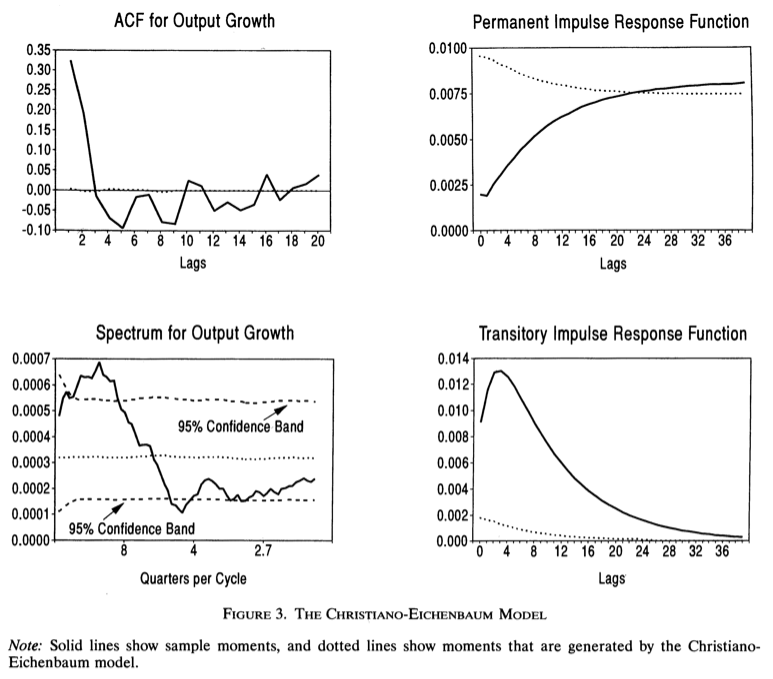
\includegraphics[width=0.57\linewidth]{figures/baseline_all.png}
        %\caption{}
    \end{figure}
    \small
    \begin{itemize}
        \item  ACF are close to zero $\Rightarrow$ No serial correlation
        \item Spectrum is quite flat $\Rightarrow$ No Business-cycle periodicity in output
              growth
        \item Some success matching the permanent IRF
        \item The model strongly damps transitory shock and generates monotonic decay
              $\Rightarrow$ No trend-reverting component in output
    \end{itemize}
\end{frame}

\subsection{Gestation Lags and Capital Adjustment Costs}

\begin{frame}{Gestation Lags and Capital Adjustment Costs}

    \begin{itemize}
        \item \textbf{Time-to-build Model}

              Firms face a 3-quarter gestation lag when installing new capital

        \item \textbf{Q-theoretic Model}

              Quadratic costs of adjusting the capital stocks

              Production function becomes: $$ \ln \left(y_t\right)= \ln \left[f\left(k_t, a_t
                      n_t\right)\right] -\left(\alpha_{k} / 2\right)\left[\Delta k_t /
                      k_{t-1}\right]^2 $$

              Based on Shapiro (1986), $\alpha_{k}$ is calibrated to be 2.2
    \end{itemize}

\end{frame}

\begin{frame}{Comparison}
    \begin{figure}
        \centering
        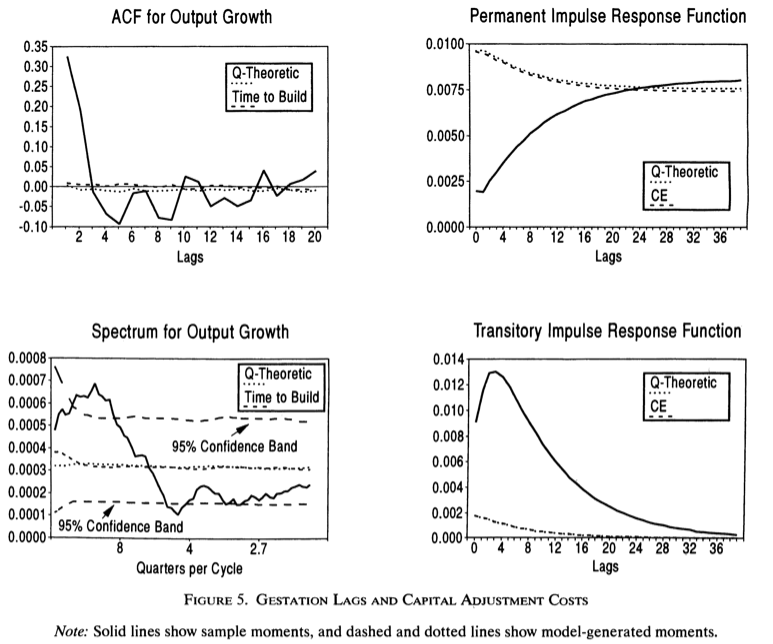
\includegraphics[width=0.65\linewidth]{figures/Capital_adj_cost.png}
        %\caption{}
    \end{figure}
    \small
    \begin{itemize}
        \item No serial correlation or Business-cycle periodicity in output growth
        \item No effect on IRF $\Rightarrow$ No help to propagate shocks
              \begin{itemize}
                  \item Gestation Lags and Capital Adjustment Costs alter $I_t$, but $I_t$ is small
                        relative to $k_t$ $\Rightarrow$ little effect on $y_t$
              \end{itemize}
    \end{itemize}

\end{frame}

\subsection{Employment Lags and Labor Adjustment Costs}
\begin{frame}{Employment Lags and Labor Adjustment Costs}
    \begin{itemize}
        \item \textbf{Adjustment-cost model}

              Production function: $$ \ln \left(y_t\right)= \ln \left[f\left(k_t, a_t
                      n_t\right)\right] -\left(\alpha_{k} / 2\right)\left[\Delta k_t /
                      k_{t-1}\right]^2 -\left(\alpha_n / 2\right)\left[\Delta n_t / n_{t-1}\right]^2
              $$

              Shapiro's estimate : $\alpha_{k} = 0.36$

        \item \textbf{Labor-hoarding model} Burnside et al. (1993)

              Firms must choose the size of the labor force before observing the current
              state of the economy but can vary the intensity of work effort after observing
              the current state
    \end{itemize}

\end{frame}

\begin{frame}{Comparison}
    \begin{figure}
        \centering
        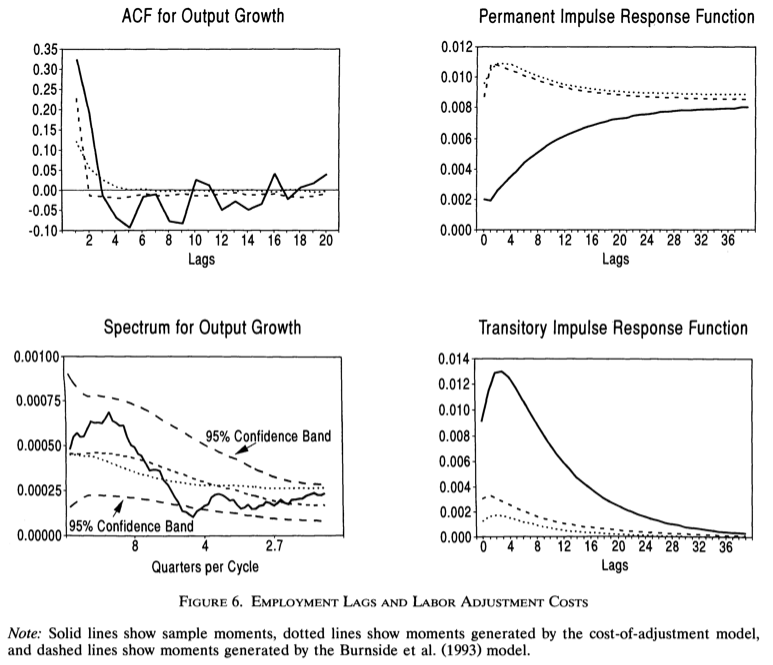
\includegraphics[width=0.57\linewidth]{figures/Labor_cost.png}
        %\caption{}
    \end{figure}
    {\footnotesize
    \begin{itemize}
        \item Positive autocorrelation at lag 1, and modest negative autocorrelation at
              higher-order lags in output growth
              % \begin{itemize}
              %     \item Burnside et al. (1993) model: positively autocorrelated at lag 1 and has modest negative autocorrelation at higher-order lags
              %     \item Adjustment-cost model: output growth is well approximated by an AR(1), with positive autocorrelation at lag 1 and monotonic decay at higher-order lags
              % \end{itemize}
        \item Modest business-cycle periodicity
        \item Overstate the short-term response of permanent shocks and understate its
              response to transitory shock
        \item No important trend-reverting component in output
    \end{itemize}}
\end{frame}

\section{Contribution}

\begin{frame}{Contribution}
    \begin{itemize}
        \item Baseline model and gestation lags and capital adjustment costs model have weak
              internal propagation mechanisms and do not generate dynamics via their internal
              structure
        \item Models that rely on lags or costs of adjusting labor input are partially
              successful:
              \begin{itemize}
                  \item Right pattern of autocorrelation in output growth
                  \item Small hump in transitory IRF
              \end{itemize}
    \end{itemize}

\end{frame}

\begin{frame}{ACF for Output Growth}
    \begin{minipage}{0.33\textwidth}
        \begin{figure}
            \centering
            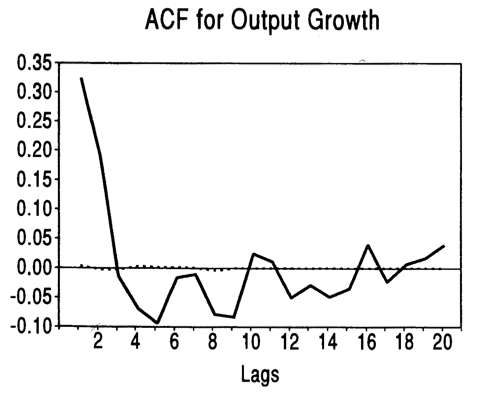
\includegraphics[width=\linewidth]{figures/Bse_ACF.png}
            \caption{Baseline Model}
        \end{figure}
    \end{minipage}%
    \begin{minipage}{0.33\textwidth}
        \begin{figure}
            \centering
            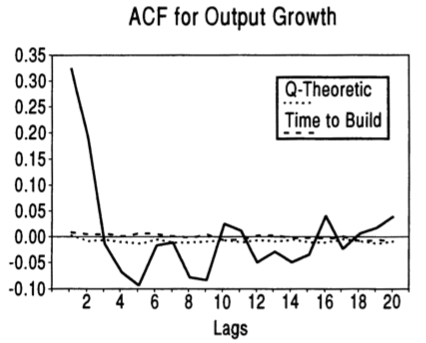
\includegraphics[width=\linewidth]{figures/K_ACF.png}
            \caption{Capital Adjustment Cost}
        \end{figure}
    \end{minipage}%
    \begin{minipage}{0.33\textwidth}
        \begin{figure}
            \centering
            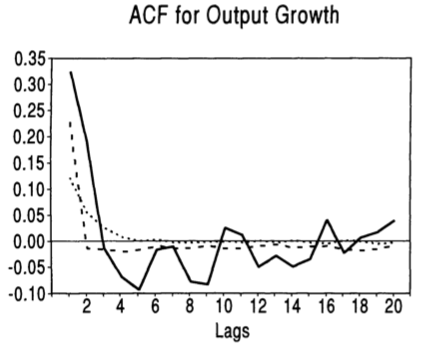
\includegraphics[width=\linewidth]{figures/L_ACF.png}
            \caption{Labor Adjustment Cost}
        \end{figure}
    \end{minipage}

    \begin{itemize}
        \item Baseline \& Capital: No serial autocorrelation
        \item Labor: Positive autocorrelation at lag 1
    \end{itemize}

\end{frame}

\begin{frame}{Spectrum for Output Growth}
    \begin{minipage}{0.33\textwidth}
        \begin{figure}
            \centering
            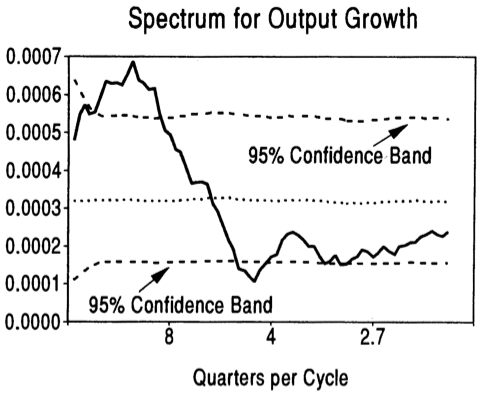
\includegraphics[width=\linewidth]{figures/Base_spect.png}
            \caption{Baseline Model}
        \end{figure}
    \end{minipage}%
    \begin{minipage}{0.33\textwidth}
        \begin{figure}
            \centering
            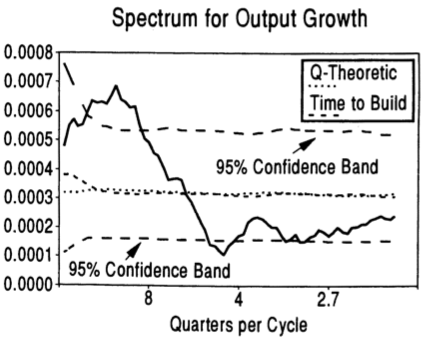
\includegraphics[width=\linewidth]{figures/K_spect.png}
            \caption{Capital Adjustment Cost}
        \end{figure}
    \end{minipage}%
    \begin{minipage}{0.33\textwidth}
        \begin{figure}
            \centering
            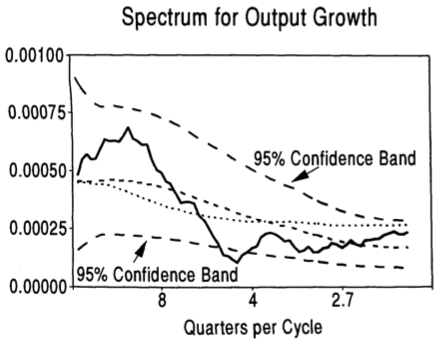
\includegraphics[width=\linewidth]{figures/L_spect.png}
            \caption{Labor Adjustment Cost}
        \end{figure}
    \end{minipage}

    \begin{itemize}
        \item Baseline \& Capital: Spectrum is quite flat $\Rightarrow$ No Business-cycle
              periodicity in output growth
        \item Labor: Modest business-cycle periodicity
    \end{itemize}

\end{frame}

\begin{frame}{Permanent Impulse Response Function}
    \begin{minipage}{0.33\textwidth}
        \begin{figure}
            \centering
            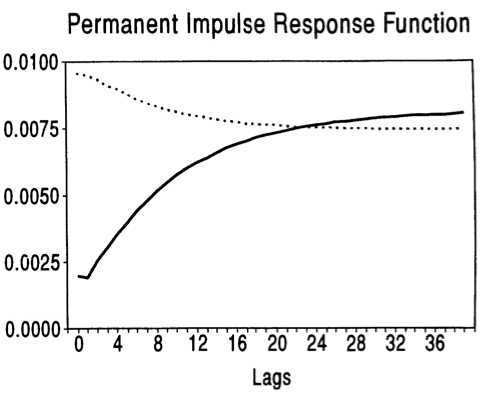
\includegraphics[width=\linewidth]{figures/Base_per_IRF.png}
            \caption{Baseline Model}
        \end{figure}
    \end{minipage}%
    \begin{minipage}{0.33\textwidth}
        \begin{figure}
            \centering
            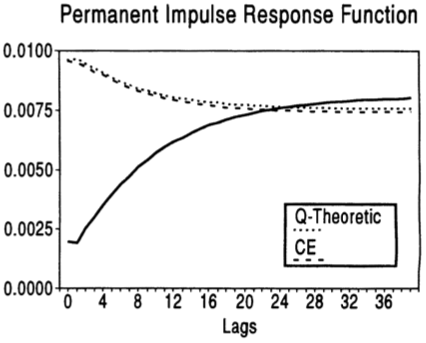
\includegraphics[width=\linewidth]{figures/K_per_IRF.png}
            \caption{Capital Adjustment Cost}
        \end{figure}
    \end{minipage}%
    \begin{minipage}{0.33\textwidth}
        \begin{figure}
            \centering
            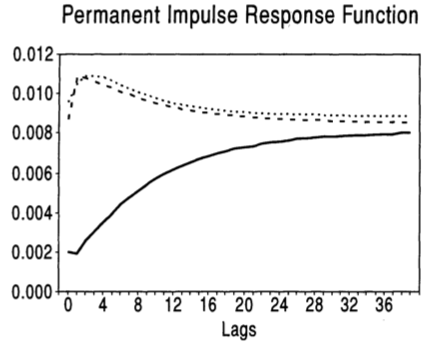
\includegraphics[width=\linewidth]{figures/L_per_IRF.png}
            \caption{Labor Adjustment Cost}
        \end{figure}
    \end{minipage}

    \begin{itemize}
        \item Baseline \& Capital: Some success in matching the permanent IRF
        \item Labor: Hump-shared response of output to technology shocks
    \end{itemize}

\end{frame}

\begin{frame}{Transitory Impulse Response Function}
    \begin{minipage}{0.33\textwidth}
        \begin{figure}
            \centering
            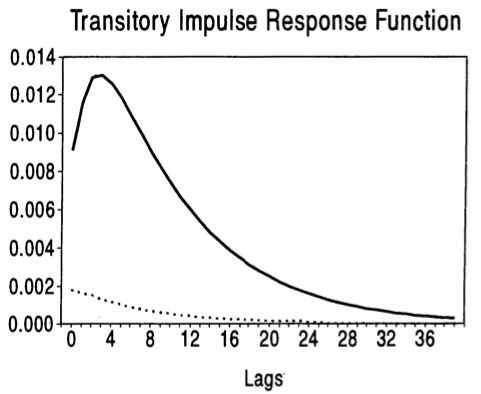
\includegraphics[width=\linewidth]{figures/Base_trans_IRF.png}
            \caption{Baseline Model}
        \end{figure}
    \end{minipage}%
    \begin{minipage}{0.33\textwidth}
        \begin{figure}
            \centering
            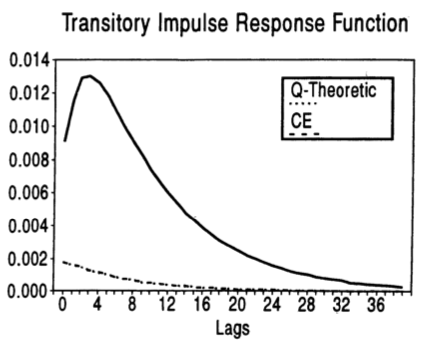
\includegraphics[width=\linewidth]{figures/K_trans_IRF.png}
            \caption{Capital Adjustment Cost}
        \end{figure}
    \end{minipage}%
    \begin{minipage}{0.33\textwidth}
        \begin{figure}
            \centering
            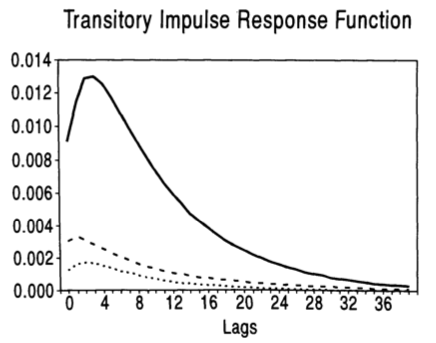
\includegraphics[width=\linewidth]{figures/L_trans_IRF.png}
            \caption{Labor Adjustment Cost}
        \end{figure}
    \end{minipage}
    \begin{itemize}
        \item Baseline \& Capital: Wrong qualitative and quantitative response to transitory
              shocks
        \item Labor: Right qualitative response to transitory shocks, but too small in
              magnitude
    \end{itemize}

\end{frame}

\begin{frame}{Refresh our memory of the course}
    RBC model with full depreciation and labor wedge, where $\z_t$ follows random walk with drift and $n_t$ follows an AR(1) process. The stochastic components share the same property with those in this paper \cite{cogley_nason_1995}.
    The model result is also balanced growth, which implies stationarity of $\Delta y_t$ and $n_t$.
\end{frame}

\begin{frame}[allowframebreaks]{References}

    \bibliography{main.bib}
    \bibliographystyle{abbrv}

\end{frame}

\end{document}
